\documentclass[double,12pt]{psutex}
\usepackage{graphicx}
\usepackage{rotating} %Package added to allow the rotation of figures and chart on a page, {sidewaysfigure} command
\usepackage{tablefootnote} %Packaged added to allow footnotes in the tabular environment, use \tablefootnote command


\usepackage{amsmath}
\usepackage{amssymb}
\usepackage{textcomp, gensymb} % for degree symbol
\usepackage[dvipsnames]{xcolor} % colorbox for inline comments
\usepackage{cite}
\usepackage{booktabs}
\usepackage{tabularx}
\usepackage[flushleft]{threeparttable}
\usepackage{dcolumn}
\usepackage{float}
\usepackage{longtable}
\usepackage{hyperref}
\usepackage{algorithm}

\newcommand{\shortnote}[1]{\footnote{\color{red}#1}}

\renewcommand{\arraystretch}{1.0}


% -------------------------------------------------
% Define variables needed to build the Title Page
% -------------------------------------------------
\title{An Unconference for the Rust of Us} % line break needs to be inserted manually for it to be double-spaced
\author{Robert Elia}
\graddegree{Bachelor of Science}
\doctype{Thesis}
\university{Portland State University}
\department{Computer Science}
\major{Computer Science}
\submitdate{_, 2026}
\commencementyear{2026}
\committeemembers{Bart Massey}

\usepackage{etoolbox} % For the flag determining if front matter goes into the TOC
\usepackage{listings}
\newtoggle{fulltoc}
\toggletrue{fulltoc}  % Change to \togglefalse{fulltoc} to remove front matter



\begin{document}

\maketitle

%-------------------------Pretext Pages----------------------------
% Abstract
\chapter*{\centerline{Abstract}}
\markboth{\MakeUppercase{Abstract}}{}
\iftoggle{fulltoc}{
  \addcontentsline{toc}{chapter}{Abstract}
}{}

An Unconference is a gathering of like-minded individuals who organize on the spot, with content driven by the collective interests and expertise of the participants. While digital conference tools are plentiful, they lack support for Unconferences, automatic scheduling, or both. UnconfRS is a full-stack web application built using Rust that enables participants to propose sessions, vote on them, and have a schedule generated using a heuristic-based local search with random restarts and simplified simulated annealing. The scheduler is evaluated against an exhaustive brute force search. The results show that it is able to find good schedules while running approximately 380 times faster than brute force on a small benchmark. These results demonstrate that local search techniques can produce good Unconference schedules. Additionally, it shows that Rust is well-suited for implementing the backend and the scheduler.

% Dedication
% \chapter*{\centerline{}}
\markboth{\MakeUppercase{Dedication}}{}
\iftoggle{fulltoc}{
  \addcontentsline{toc}{chapter}{Dedication}
}{}

\begin{center}
\emph{[Lorem Ipsum]}
\end{center}


% Acknowledgements
\chapter*{\centerline{Acknowledgments}}
\markboth{\MakeUppercase{Acknowledgments}}{}
\iftoggle{fulltoc}{
  \addcontentsline{toc}{chapter}{Acknowledgments}
}{}
I want to express my deepest thanks to my thesis advisor, Dr. Bart Massey. My first class with Bart was Embedded Rust, in that class my curiosity was encouraged and I was challenged to pursue many of these curiosities with guidance. That encouragement carried over into this thesis, where his expertise, guidance, and feedback helped shape the direction of this project.

I would like to express my sincere gratitude to my partner, Megan. Her support was instrumental for me to succeed as a returning student, from celebrating my wins to providing encouragement when things were tough. Megan was always there for me.

I want to thank my friends and family who believed in me and encouraged me in my journey.

%-------------------------Listings-----------------------------
% Table of contents, list of figures, etc
% Manually uncomment the listings for types that are present in the document
\tableofcontents
\listoftables
\listoffigures
% \listofnomenclatures
% \listofappendices
% \listofappendixfigures
% \listofappendixtables

%-------------------------Main Chapters-----------------------------
\mainmatter

\chapter{Introduction}
Imagine a typical conference: you have a printed program with scheduled talks, audience members quietly sitting in rows, and experts with rehearsed presentations at the front. Now, instead imagine that you walk into a room with blank scheduling boards, no predetermined talks, and participants actively creating the conference agenda. This on-the-fly event is an Unconference.

These Unconferences have gained popularity in academic, technology, and professional communities for their ability to facilitate knowledge exchange. Unconferences have emerged as an alternative to traditional conference formats. Based on Open Space Technology principles, Unconferences follow a structure that involves collaborative agenda creation, breakout sessions, and collective sharing of insights. Chapter 2 goes further in depth on Unconferences.

However, Unconferences present challenges that existing event management tools designed for traditional conferences fail to address effectively. Although Unconferences rely on simple materials such as flipboards, markers, and post-it notes, there is a gap in digital solutions that can support the participant-driven and on-the-spot organizing of Unconferences. More specifically, scheduling sessions that capture participant preferences is a challenging problem, even for smaller Unconferences. Existing conference software does not seem to support this automated scheduling that captures participant preferences.

This thesis presents UnconfRS, a digital platform designed to support the needs of Unconference organizers and participants. Specifically, this work looks to answer whether modern scheduling techniques can be used to create an effective Unconference management tool and whether Rust is an effective language for implementing the backend and the scheduler. By addressing these questions, this work aims to provide a tool that can effectively manage Unconferences.
%
%
\chapter{Understanding Unconferences}
This chapter defines what an Unconference is, briefly covering its origins, and describing what happens during a typical Unconference. These insights directly influence UnconfRS. Understanding Unconferences helps create a tool to aid in organizing them.

\section{Defining Unconferences}
An Unconference is a gathering of like-minded individuals who organize on the spot. The content of the Unconference is driven by the collective interests and expertise of the participants\cite{budd2015, duke2022}. In contrast, the typical conference is planned well in advance by few people, with the speakers, topics, and timing already determined. When presentations happen, there is an expectation for people to remain seated, listen, and hold questions until the end.

Unconferences tend to draw upon Open Space Technology (OST), a specific format of Unconference developed by Harrison Owen in the 1980s after the conclusion of the conference he put on revealed that the most useful parts were the coffee breaks \cite{harrison2008}. Some may use "Unconference" and "OST" interchangeably, but these are not the same. OST is a specific way of organizing and facilitating, while Unconference is a broader term not tied to a specific format. OST can be understood as an influential and popular type of Unconference. An OST meeting starts with participants in a circle with a blank agenda. Then they perform the agenda-setting exercise, putting their ideas on the wall (community bulletin board). After that, people gather in small groups (marketplace) for the ideas they are most interested in.\cite{harrison2008}

Some notable Unconferences include Foo Camp, Bar Camp, Ed Camp, and GSoC (Google Summer of Code) Mentor Summit. Foo Camp is an invitation-only event focused on computer science that started in 2003\cite{oreilly2018}. Bar Camp came about as an open alternative to Foo Camp in 2005 after Tantek Celik hadn't (yet) received an invitation to Foo Camp\cite{celik2006}. Ed Camp adopted the Unconference model for educators for professional development\cite{edcamp2011}. GSoC Mentor Summit adopted the Unconference model for bringing together mentors following the conclusion of that year's GSoC program\cite{googleblog2006}.

\section{A Typical Unconference}
A typical Unconference has three phases: agenda creation, breakout sessions, and gathering together. Agenda creation involves participants proposing session topics, usually written on post-it notes or index cards placed on a flipboard or whiteboard. Once the agenda is created and scheduled, these breakout sessions discuss the proposed topics. The event concludes with reconvening to share what has been learned.

Breakout sessions are distributed across multiple rooms and run in short consecutive timeslots. Multiple sessions are run in parallel, with participants being able to move freely between them. The schedule is posted visibly, allowing attendees to plan which sessions to attend.

Results are captured through session notes taken during discussions. At the closing gathering, attendees summarize sessions and share what they've learned throughout the experience.
\chapter{Related Work}\label{ch:related Work}

\section{Existing Unconference Platforms}
Pretalx \cite{kunze2017} is a full-featured open-source conference management tool that handles submission and review, selection, and scheduling of sessions. It also has an extension ecosystem that could support the participant-driven session proposals and voting used in Unconferences. However, while its scheduling features are extensive, schedule construction is a manual process. UnconfRS automates schedule generation.

The Xen Project session-scheduler \cite{dunlap2018} is the most comparable existing tool to UnconfRS. It is an open-source web application for scheduling Unconference sessions written in Go. It enables users to propose sessions, express a level of interest in each session, and have schedules generated that maximize participation. UnconfRS, which is written in Rust, shares much of this. It also has these goals: have desirable sessions happen earlier in the day, avoid concurrent sessions on the same topic, minimize overlap of popular sessions, and reduce conflicts where speakers miss sessions they wanted to attend due to them leading another session at the same time. Additionally, UnconfRS utilizes local search for the scheduling.

\section{Scheduling Approaches}
Kim et al. \cite{kim2013} introduced Cobi, a community-informed conference scheduling tool at CHI 2013. Cobi utilizes community input in the form of schedule preferences and constraints. Using constraint-solving provides organizers with context for the state of the current schedule, such as if there are session conflicts and can provide suggestions for how to best improve the schedule. However, this is an intentional manual process. UnconfRS opts for schedule generation to utilize community input to generate a schedule, but allow manual tweaks for fine tuning. 

Riquelme et al. \cite{riquelme2022} compared using a Gurobi solver and a heuristic method based on simulated annealing for solving a track-based conference scheduling problem. They found that when the Gurobi solver was able to find optimal solutions, the simulated annealing approach was able to find solutions quicker. In situations where Gurobi solver was not able to find a solution in time, the simulated annealing approach found near-optimal solutions. UnconfRS similarly utilizes local search with simulated annealing to find good solutions quickly.


%Rezaeinia et al. \cite{rezaeinia2024}
%Scheduling conferences using data on attendees’ preferences
%\url{https://doi.org/10.1080/01605682.2024.2310722}
\chapter{Scheduling}
Why is scheduling such a big deal? Just brute force it and call it a day, should be as simple as that, right? The answer to that is a resounding no!

The scheduling problem we are dealing with here is deceptively large, even for small Unconferences. Take a small example: three rooms, five time slots, and twenty-one potential sessions to schedule. There are $\binom{n}{k}$ combinations for which sessions will be scheduled, where n is the total number of sessions and k is the capacity of the schedule $\binom{21}{15}=54,264$. Then for each of these combinations there are $\frac{n!}{k_1! \cdot k_2! \cdot k_3! \cdot k_4 \cdot k_5}$ ways to group the sessions across the 5 timeslots, where n is the number of sessions to schedule and $k_1$, $k_2$, $k_3$, $k_4$, and $k_5$ are the capacities of the 5 timeslots. In this schedule that works out to $\frac{15!}{3! \cdot 3! \cdot 3! \cdot 3! \cdot 3!}=168,168,000$. This means the total number of possible schedules is $num\_combinations \cdot ways\_to\_group$, or $54,264 \cdot 168,168,000=9,125,468,352,000$ possibilities for our scheduler to create and score just to determine the best schedule. At this size the problem is already getting too large to brute force in a reasonable amount of time. 

\section{Search}
There are several search concepts to consider: informed search (search that leverages heuristics: functions that indicate how good or close to the goal state they are), uninformed search (does not leverage information to guide it toward the goal), complete search (guaranteed to eventually find the goal), systematic search (guaranteed to find the goal without re-visiting any states), stochastic search (randomized, so not guaranteed to ever find the goal), local search (a common and effective kind of stochastic search), and anytime property (able to stop at any point and return the best solution so far, with longer runtime leading to better results and eventually optimality).

The problem with brute force search is that it is an uninformed systematic search that explores areas that move it away from the goal. If brute force is not a reasonable solution, how do we go about scheduling? That depends on our goals for scheduling. If the goal is to determine whether a solution exists or to find the optimal solution, then a complete or systematic search would work well. However, for UnconfRS, the goal is to find a reasonably good solution quickly. This makes informed local search a good fit since it lends itself to the anytime property, allowing the scheduler to return the best solution found so far.
%
%
\section{Local Search}
The local search used in this project works by starting at an initial candidate solution and iteratively moving to neighboring states in the search space (the set of all unique solutions). A neighbor (a different candidate solution from a single small move in the previous state) for UnconfRS would be swapping a session with another, either already on the schedule or with one that is unassigned.

At each step, the neighborhood (the set of all neighbors from the current state) is evaluated using heuristic functions. A neighbor is then chosen to explore. Which neighbor is chosen depends on the local search algorithm, ranging from greedy (best improving) to stochastic. This continues until reaching a local minimum (candidate solution is better than all its neighbors). It is possible it is also a global minimum (candidate solution better than all others in the search space). However, there is no guarantee of finding a global minimum using local search.

Random restarts and noise moves are strategies that can be used to avoid getting trapped in a non-global minimum. With random restarts, the scheduling is run many times from different randomly initialized starting states. Noise moves are random moves that attempt to prevent the search from getting stuck in a local minimum.
\chapter{An Unconference Software Solution}
\section{UnconfRS}
UnconfRS is a full stack web application that allows users to propose sessions and vote on sessions they are interested in. They can also view a populated schedule that contains information about the session and where the session is located. Additionally there is functionality for admin and facilitators to make edits to sessions others have submitted (e.g. choosing a more appropriate tag for a session). The admin alone can generate a schedule which uses the known information of who is putting on a session at a specific time and which sessions users expressed interest in to attempt to create a best schedule. The admin also has fine control with being able to drag and drop the sessions already on the schedule. 
\subsection{Creating an agenda}
There are three main steps for a user to participate in agenda creation: registering a new account through the UnconfRS website, proposing sessions on the sessions page, and voting on sessions they would like to attend.\\

\subsection{Scheduling For UnconfRS}
Once an agenda has been created, the admin needs to create the schedule. The first step in that process is clicking the button Populate Schedule on the unconf schedule page. This attempts to create a best schedule that avoids conflicts and tries to make sure people are able to see the sessions they want. At this point the admin can make manual changes to the schedule as well. They can remove or add to the schedule, as well as drag and drop sessions on the schedule to move when the sessions are happening.\\

\section{Implementation}
This section describes the technical decisions for the implementation of UnconfRS. From the choice of Rust as the programming language, system design and architecture, frontend, backend, database, security, and the scheduling approach.

\subsection{Why Rust}
Rust was chosen because it is a modern programming language that provides performance, reliability, and productivity. The scheduler needs to evaluate many candidate solutions quickly, so a performant language was desired. The type system and ownership model ensure many potential bugs are caught at compile time. Additionally, the existing ecosystem of crates meets the majority of the needs for this project.
%"https://rust-lang.org/"\\
%Performance, Reliability, Productivity
\subsection{System Design and Architecture}
The makeup of UnconfRS can be divided up into three main parts consisting of a Rust-based backend (Axum), PostgreSQL database (SQLx), and a mostly server-side rendered frontend (Askama) with JavaScript enhancements.\\
\\The project is organized as three Cargo workspaces: \texttt{server}, \texttt{scheduler}, and \texttt{test data creation}. The \texttt{server} workspace contains all aspects relating to the frontend, backend, and database. The \texttt{scheduler} workspace contains the scheduling library that gets used when generating a schedule. The \texttt{test data creation} workspace contains a utility for generating test data. Having the separate workspaces makes it clear what the code in the workspace is responsible for. It also has the benefit of lowering compilation time.\\
\\Overall the web application follows an MVC (Model View Controller) architecture design pattern, where models manage data/business logic, views handle the user interface, and controllers act as an intermediary between models and views. This pattern provides a straightforward way for separating code according to specific responsibilities.
\begin{figure}[h]
    \centering
    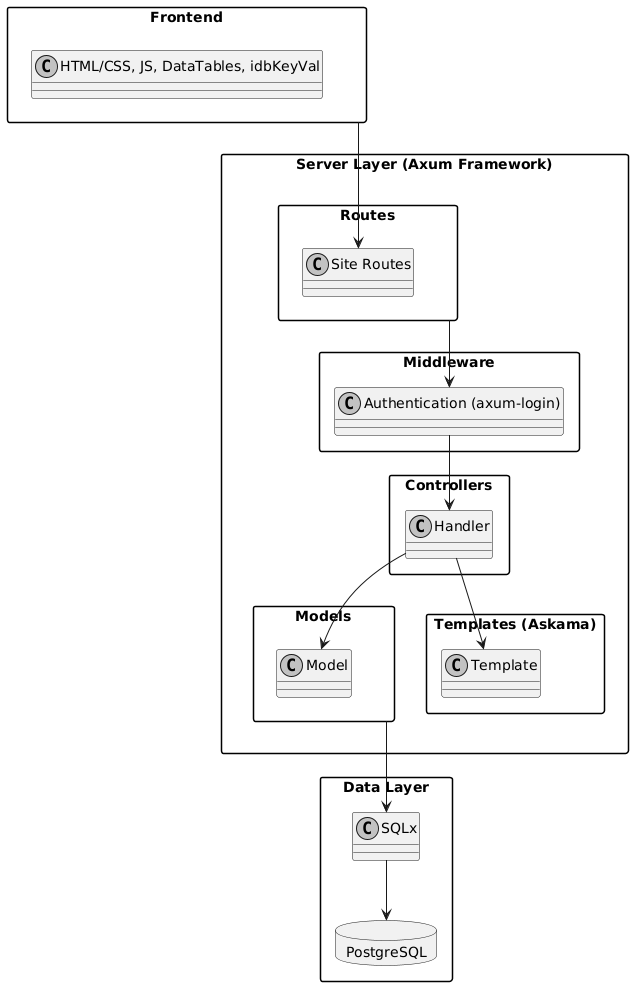
\includegraphics[width=0.85\linewidth]{figs/high_level_diagram.png}
    \caption{High level diagram showing the different areas of implementation}
    \label{fig:enter-label}
\end{figure}
\clearpage
\subsection{Frontend}
The frontend utilizes Askama for server-side template rendering, chosen for its compile time type safety. DataTables is used for displaying the table of sessions in a responsive and interactive manner. Bootstrap 5.3.8 is utilized for responsive styling. The HTML 5 Drag and Drop API is used to allow for schedule manipulation. For client-side storage, IDB-Keyval is used.

\subsection{Backend}
The backend is built with Axum (by Tokio), which is a web application framework written in Rust that focuses on ergonomics and modularity. It uses the Tokio async runtime for concurrent I/O. Axum was chosen here due to prior familiarity and its growing adoption in the Rust community. For middleware and authentication/authorization various Tower crates and axum-login are used. For serializing and deserializing data structures Serde is used.

\subsection{Database}
For the database, PostgreSQL was chosen mostly due to prior familiarity, but it is also a powerful open source relational database system. For working with the database in the backend, the crate SQLx was chosen. This was chosen due to it featuring compile time checked queries.

\subsection{Security Considerations}
UnconfRS implements session-based authentication and role-based authorization for access to the application.\\\\
\textbf{Authentication}:
The application uses axum-login for session-based authentication. The passwords are stored hashed using bcrypt.\\
Login workflow:
\begin{enumerate}
    \item User submits Unconference password in order to access the site
    \item On success a server-side session is created in PostgreSQL
    \item Session ID is stored in a secure HTTP only cookie
    \item User submits credentials in the account login form
    \item On success a new session associated to the logged in user replaces the one for site access (in the database and in the cookie)
\end{enumerate}

\textbf{Authorization}:
Permission based access is implemented also using axum-login with different levels of access:

\begin{table}[hbtp]
    \centering
    \begin{tabular}{|m{12em}| ccccc|}
      \hline
     ~ & \multicolumn{2}{|c}{Unauthorized} & \multicolumn{3}{c|}{Authorized} \\
     \hline
     Scenarios & Public & User & User & Staff & Admin\\
     \hline
         Unconf login page &  \checkmark & \checkmark & \checkmark & \checkmark & \checkmark\\
         \hline
         Read-only site access & X & \checkmark & \checkmark & \checkmark & \checkmark\\
         \hline
         CRUD actions on their own sessions & X & X & \checkmark & \checkmark & \checkmark\\
         \hline
         Voting on sessions & X & X & \checkmark & \checkmark & \checkmark\\
         \hline
         CRUD actions on any sessions & X & X & X & \checkmark & \checkmark\\
         \hline
         Create session for a user & X & X & X & \checkmark & \checkmark\\
         \hline
         Register user on their behalf & X & X & X & \checkmark & \checkmark\\
         \hline
         CRUD actions for tags & X & X & X & X & \checkmark \\
         \hline
         Schedule setup (adding rooms and timeslots) & X & X & X & X & \checkmark \\
         \hline
         Manipulating the schedule (adding/removing sessions to the schedule or running the scheduler) & X & X & X & X & \checkmark \\
         \hline
    \end{tabular}
    \caption{Actions unauthorized/authorized users can take depending on their role}
    \label{tab:placeholder}
\end{table}
\FloatBarrier
%\begin{itemize}
%    \item \textbf{User} (default): Can submit sessions, update/delete sessions %they created, vote for sessions, and view the schedule
%    \item \textbf{Facilitator} (staff): Can do all that a User can, but they can %also create sessions on behalf of a user, make edits to any session, and register %a user on their behalf, 
%    \item \textbf{Admin} (superuser): Can do all that Staff can, but they can %also create/update/delete the tags that sessions can use, perform the setup for %the schedule (adding rooms and timeslots), and manipulation of the schedule %(adding sessions manually or running the scheduler).
%\end{itemize}

%How the application utilizes authorization and authentication:
%\begin{itemize}
%    \item \textbf{Routes}: Routes are broken up into 5 parts:
%    \begin{itemize}
%        \item No Unconference authentication (can only access Unconference login)
%        \item Unconference authentication but no account authentication (read %only view with User level permissions)
%        \item Unconference authentication and account authentication at User %permission level (read/write access with User level permissions)
%        \item Unconference authentication and account authentication at %Facilitator permission level (read/write access with Facilitator level %permissions)
%        \item Unconference authentication and account authentication at Admin %permission level (read/write access with Admin level permissions)
%    \end{itemize}
%    \item \textbf{Middleware}: Routes utilize middleware to ensure users have the %specified permissions
%    \item \textbf{Ownership}: The application makes sure sessions can only be %updated by the users that created them or by Admin/Facilitators
%    \item \textbf{Askama Templating}: By passing the Askama templates the %permission levels we can conditionally include source files that require higher %level of permissions
%\end{itemize}
\subsection{Scheduling}
As mentioned in the previous scheduling chapter, trying to create schedules for Unconferences creates a state space that would take an unreasonable amount of time to search. The application has access to data so instead of an uninformed brute force search an informed search can be done. The scheduler has access to the number of votes each session received, session tag ID, session speaker ID, and which sessions each speaker voted for. Having that information, heuristics can be created to apply a score to the schedule, where the score is a collection of penalties assessed based on the data. Then we can use local search for the strategy on trying to find the best schedule.

\subsubsection{Heuristics}
For the scheduler the heuristics are made up of five penalty functions that assess scores based on scenarios that lead to a worse schedule. \\\\
%
%
\textbf{Penalize Conflicting Popular Sessions}: For each timeslot, it sorts the sessions, then sums the products of adjacent pairs by their vote counts. This ends up with higher scores for schedules that have high vote sessions happening at the same time as other high vote sessions.
\begin{pseudocode}{Penalty for concurrent popular sessions}
    %\begin{tabbing}Penalty {\bf for} multiple concurrent popular sessions across $Timeslots$$:$\\
%$~~~~$$popular\_conflict$ $\leftarrow$ $0$\\
%$~~~~${\bf for} $i$ {\bf in} $0..$length($Timeslots$)$-1$\\
%$~~~~~~~~$$sorted$ $\leftarrow$ sort $Timeslots$$[$$i$$]$ by votes descending\\
%$~~~~~~~~$$popular\_conflict\_slot$ $\leftarrow$ $0$\\
%$~~~~~~~~${\bf for} $j$ {\bf in} $0..$length($sorted$)$-2$\\
%$~~~~~~~~~~~~$$popular\_conflict\_slot$ $\leftarrow$ $popular\_conflict\_slot$ $+$ $sorted$$[$$j$$]$ %$*$ $sorted$$[$$j$ $+$ $1]$\\
%$~~~~~~~~$$popular\_conflict$ $\leftarrow$ $popular\_conflict$ $+$ $popular\_conflict\_slot$\\
%$~~~~${\bf return} $popular\_conflict$\\
%\end{tabbing}
\begin{tabbing}Penalty {\bf for} multiple concurrent popular sessions across $\textit{Timeslots}$$:$\\
$~~~~$$\textit{popular\_conflict}$ $\leftarrow$ $0$\\
$~~~~${\bf for} $\textit{i}$ {\bf in} $0..$length($\textit{Timeslots}$)$-1$\\
$~~~~~~~~$$\textit{sorted}$ $\leftarrow$ sort $\textit{Timeslots}$$[$$\textit{i}$$]$ by votes descending\\
$~~~~~~~~$$\textit{popular\_conflict\_slot}$ $\leftarrow$ $0$\\
$~~~~~~~~${\bf for} $\textit{j}$ {\bf in} $0..$length($\textit{sorted}$)$-2$\\
$~~~~~~~~~~~~$$\textit{popular\_conflict\_slot}$ $\leftarrow$ $\textit{popular\_conflict\_slot}$ $+$ $\textit{sorted}$$[$$\textit{j}$$]$ $*$ $\textit{sorted}$$[$$\textit{j}$ $+$ $1]$\\
$~~~~~~~~$$\textit{popular\_conflict}$ $\leftarrow$ $\textit{popular\_conflict}$ $+$ $\textit{popular\_conflict\_slot}$\\
$~~~~${\bf return} $\textit{popular\_conflict}$\\
\end{tabbing}
\end{pseudocode}

\textbf{Penalize Popular Session Missing}: This penalty function goes through every scheduled session and compares it with every unscheduled session. For every unscheduled session that has more votes than the scheduled one, a penalty is added proportional to the difference of votes.
\begin{pseudocode}{Penalty for popular sessions missing from the schedule}
    % \begin{tabbing}Penalty {\bf for} sessions {\bf in} $Unassigned\_Sessions$ list more popular than {\bf in} $Assigned\_Sessions$ list$:$\\
% $~~~~$$missing\_popular\_sessions$ $\leftarrow$ $0$\\
% $~~~~${\bf for} each $Assigned$ session {\bf in} $Assigned\_Sessions$$:$\\
% $~~~~~~~~$$missing\_popular\_sessions\_slot$ $\leftarrow$ $0$\\
% $~~~~~~~~${\bf for} each $Unassigned$ session {\bf in} $Unassigned\_Sessions$$:$\\
% $~~~~~~~~~~~~${\bf if} $Unassigned$ $>$ $Assigned$\\
% $~~~~~~~~~~~~~~~~$$difference$ $\leftarrow$ $Unassigned$ $-$ $Assigned$\\
% $~~~~~~~~~~~~~~~~$$missing\_popular\_sessions\_slot$ $\leftarrow$ $missing\_popular\_sessions\_slot$ $+$ $difference$\\
% $~~~~~~~~$$missing\_popular\_sessions\_slot$ $\leftarrow$ $missing\_popular\_sessions\_slot$ $*$ $15$\\
% $~~~~~~~~$$missing\_popular\_sessions$ $\leftarrow$ $missing\_popular\_sessions$ $+$ $missing\_popular\_sessions\_slot$\\
% $~~~~${\bf return} $missing\_popular\_sessions$\\
% \end{tabbing}
\begin{tabbing}Penalty {\bf for} sessions {\bf in} $\textit{Unassigned\_Sessions}$ list more popular than {\bf in} $\textit{Assigned\_Sessions}$ list$:$\\
$~~~~$$\textit{missing\_popular\_sessions}$ $\leftarrow$ $0$\\
$~~~~${\bf for} each $\textit{Assigned}$ session {\bf in} $\textit{Assigned\_Sessions}$$:$\\
$~~~~~~~~$$\textit{missing\_popular\_sessions\_slot}$ $\leftarrow$ $0$\\
$~~~~~~~~${\bf for} each $\textit{Unassigned}$ session {\bf in} $\textit{Unassigned\_Sessions}$$:$\\
$~~~~~~~~~~~~${\bf if} $\textit{Unassigned}$ $>$ $\textit{Assigned}$\\
$~~~~~~~~~~~~~~~~$$\textit{difference}$ $\leftarrow$ $\textit{Unassigned}$ $-$ $\textit{Assigned}$\\
$~~~~~~~~~~~~~~~~$$\textit{missing\_popular\_sessions\_slot}$ $\leftarrow$ $\textit{missing\_popular\_sessions\_slot}$ $+$ $\textit{difference}$\\
$~~~~~~~~$$\textit{missing\_popular\_sessions\_slot}$ $\leftarrow$ $\textit{missing\_popular\_sessions\_slot}$ $*$ $15$\\
$~~~~~~~~$$\textit{missing\_popular\_sessions}$ $\leftarrow$ $\textit{missing\_popular\_sessions}$ $+$ $\textit{missing\_popular\_sessions\_slot}$\\
$~~~~${\bf return} $\textit{missing\_popular\_sessions}$\\
\end{tabbing}
\end{pseudocode}

\textbf{Penalize Late Popular Sessions}: For each timeslot, it sorts the sessions, then sums the products of adjacent pairs by their vote counts. Each timeslot sum is multiplied by timeslot index before being added to the total sum. This ends up with popular sessions that happen later in the day incurring a larger penalty.
\begin{pseudocode}{Penalty for popular sessions occurring later in the day.}
    % \begin{tabbing}Penalty {\bf for} late popular sessions {\bf in} $Timeslots$$:$\\
% $~~~~$$late\_popular\_sessions$ $\leftarrow$ $0$\\
% $~~~~${\bf for} $i$ {\bf in} $0..$length($Timeslots$)$-1$\\
% $~~~~~~~~$$sorted$ $\leftarrow$ sort $Timeslots$$[$$i$$]$ by votes descending\\
% $~~~~~~~~$$late\_popular\_sessions\_slot$ $\leftarrow$ $0$\\
% $~~~~~~~~${\bf for} $j$ {\bf in} $0..$length($sorted$)$-2$\\
% $~~~~~~~~~~~~$$late\_popular\_sessions\_slot$ $\leftarrow$ $late\_popular\_sessions\_slot$ $+$ $sorted$$[$$j$$]$ $*$ $sorted$$[$$j$ $+$ $1]$\\
% $~~~~~~~~$$late\_popular\_sessions$ $\leftarrow$ $late\_popular\_sessions$ $+$ $late\_popular\_sessions\_slot$ $*$ $i$\\
% $~~~~${\bf return} $late\_popular\_sessions$\\
% \end{tabbing}
\begin{tabbing}Penalty {\bf for} late popular sessions {\bf in} $\textit{Timeslots}$$:$\\
$~~~~$$\textit{late\_popular\_sessions}$ $\leftarrow$ $0$\\
$~~~~${\bf for} $\textit{i}$ {\bf in} $0..$length($\textit{Timeslots}$)$-1$\\
$~~~~~~~~$$\textit{sorted}$ $\leftarrow$ sort $\textit{Timeslots}$$[$$\textit{i}$$]$ by votes descending\\
$~~~~~~~~$$\textit{late\_popular\_sessions\_slot}$ $\leftarrow$ $0$\\
$~~~~~~~~${\bf for} $\textit{j}$ {\bf in} $0..$length($\textit{sorted}$)$-2$\\
$~~~~~~~~~~~~$$\textit{late\_popular\_sessions\_slot}$ $\leftarrow$ $\textit{late\_popular\_sessions\_slot}$ $+$ $\textit{sorted}$$[$$\textit{j}$$]$ $*$ $\textit{sorted}$$[$$\textit{j}$ $+$ $1]$\\
$~~~~~~~~$$\textit{late\_popular\_sessions}$ $\leftarrow$ $\textit{late\_popular\_sessions}$ $+$ $\textit{late\_popular\_sessions\_slot}$ $*$ $\textit{i}$\\
$~~~~${\bf return} $\textit{late\_popular\_sessions}$\\
\end{tabbing}
\end{pseudocode}

\textbf{Penalize Same Topic Timeslots}: This penalty function iterates each of the timeslots. Within each timeslot, construct a HashMap that tracks for each tag\_id the total votes and number of occurrences. For every item in the HashMap add to the penalty score equal to $votes$ $*$ $($$count$ $-$ $1$$)$.
\begin{pseudocode}{Penalty for multiple sessions in the same timeslot having the same topic.}
    % \begin{tabbing}Penalty {\bf for} concurrent $sessions$ with same $tag\_id$ {\bf in} $Timeslots$$:$\\
% $~~~~$$tag\_counts$ $\leftarrow$ initialize empty HashMap of $tag\_id$ $\rightarrow$ ($votes$$,$ $count$)\\
% $~~~~$$tag\_conflict$ $\leftarrow$ $0$\\
% $~~~~${\bf for} $timeslot$ {\bf in} $Timeslots$\\
% $~~~~~~~~$$tag\_counts$ $\leftarrow$ reset the HashMap each iteration\\
% $~~~~~~~~$\\
% $~~~~~~~~${\bf for} $session$ {\bf in} $timeslot$\\
% $~~~~~~~~~~~~${\bf if} $session$$.$$session\_id$ and $session$$.$$tag\_id$ exist\\
% $~~~~~~~~~~~~~~~~$$tag\_counts$$[$$session$$.$$tag\_id$$].$$votes$ $\leftarrow$ $tag\_counts$$[$$session$$.$$tag\_id$$].$$votes$ $+$ $session$$.$$num\_votes$\\
% $~~~~~~~~~~~~~~~~$$tag\_counts$$[$$session$$.$$tag\_id$$].$$count$ $\leftarrow$ $tag\_counts$$[$$session$$.$$tag\_id$$].$$count$ $+$ $1$\\
% \\
% $~~~~~~~~${\bf for} ($votes$$,$ $count$) {\bf in} $tag\_counts$ values\\
% $~~~~~~~~~~~~$$tag\_conflict$ $\leftarrow$ $tag\_conflict$ $+$ $votes$ $*$ ($count$ $-$ $1$)\\
% $~~~~${\bf return} $tag\_conflict$\\
% \end{tabbing}
\begin{tabbing}Penalty {\bf for} concurrent sessions with same $\textit{tag\_id}$ {\bf in} $\textit{Timeslots}$$:$\\
$~~~~$$\textit{tag\_counts}$ $\leftarrow$ initialize empty HashMap of $\textit{tag\_id}$ $\rightarrow$ ($\textit{votes}$$,$ $\textit{count}$)\\
$~~~~$$\textit{tag\_conflict}$ $\leftarrow$ $0$\\
$~~~~${\bf for} $\textit{timeslot}$ {\bf in} $\textit{Timeslots}$\\
$~~~~~~~~$$\textit{tag\_counts}$ $\leftarrow$ reset the HashMap each iteration\\
\\
$~~~~~~~~${\bf for} $\textit{session}$ {\bf in} $\textit{timeslot}$\\
$~~~~~~~~~~~~${\bf if} $\textit{session}$$.$$\textit{session\_id}$ and $\textit{session}$$.$$\textit{tag\_id}$ exist\\
$~~~~~~~~~~~~~~~~$$\textit{tag\_counts}$$[$$\textit{session}$$.$$\textit{tag\_id}$$].$$\textit{votes}$ $\leftarrow$ $\textit{tag\_counts}$$[$$\textit{session}$$.$$\textit{tag\_id}$$].$$\textit{votes}$ $+$ $\textit{session}$$.$$\textit{num\_votes}$\\
$~~~~~~~~~~~~~~~~$$\textit{tag\_counts}$$[$$\textit{session}$$.$$\textit{tag\_id}$$].$$\textit{count}$ $\leftarrow$ $\textit{tag\_counts}$$[$$\textit{session}$$.$$\textit{tag\_id}$$].$$\textit{count}$ $+$ $1$\\
\\
$~~~~~~~~~~~~${\bf for} ($\textit{votes}$$,$ $\textit{count}$) {\bf in} $\textit{tag\_counts}$ values\\
$~~~~~~~~~~~~~~~~$$\textit{tag\_conflict}$ $\leftarrow$ $\textit{tag\_conflict}$ $+$ $\textit{votes}$ $*$ ($\textit{count}$ $-$ $1$)\\
$~~~~${\bf return} $\textit{tag\_conflict}$\\
\end{tabbing}
\end{pseudocode}

\textbf{Penalize Speaker Voting Conflicts}: This penalty function iterates each of the timeslots. For each session, check whether the session's speaker has voted on sessions happening at the same time. For each session happening at the same time that received a vote add to the penalty score the product of the two session vote amounts.
\begin{pseudocode}{Penalty for sessions a speaker has voted for occurring while they are scheduled for leading a session.}
    % \begin{tabbing}Penalty {\bf for} concurrent $sessions$ that conflict with $sessions$ the speaker voted {\bf for} {\bf in} $Timeslots$$:$\\
% $~~~~$$speaker\_conflict$ $\leftarrow$ $0$\\
% $~~~~${\bf for} $i$ {\bf in} $0..$length($Timeslots$) $-$ $1$\\
% $~~~~~~~~$$sessions$ $\leftarrow$ list of $sessions$ at $Timeslots$$[$$i$$]$\\
% $~~~~~~~~$$num\_sessions$ $\leftarrow$ length($sessions$)\\
% $~~~~~~~~$$speaker\_conflict\_slot$ $\leftarrow$ $0$\\
% $~~~~~~~~${\bf for} $j$ {\bf in} $0..$$num\_sessions$ $-$ $1$\\
% $~~~~~~~~~~~~$$speaker\_votes$ $\leftarrow$ the list of $sessions$$[$$j$$].$$speaker\_votes$\\
% $~~~~~~~~~~~~${\bf for} $k$ {\bf in} $0..$$num\_sessions$ $-$ $1$\\
% $~~~~~~~~~~~~~~~~${\bf if} $k$ $!=$ $j$\\
% $~~~~~~~~~~~~~~~~~~~~${\bf if} $sessions$$[$$j$$].$$session\_id$ {\bf in} $speaker\_votes$\\
% $~~~~~~~~~~~~~~~~~~~~~~~~$$session\_j\_votes$ $\leftarrow$ max($sessions$$[$$j$$].$votes$,$ $1$)\\
% $~~~~~~~~~~~~~~~~~~~~~~~~$$session\_k\_votes$ $\leftarrow$ max($sessions$$[$$k$$].$votes$,$ $1$)\\
% $~~~~~~~~~~~~~~~~~~~~~~~~$$speaker\_conflict\_session$ $\leftarrow$ $session\_j\_votes$ $*$ $session\_k\_votes$\\
% $~~~~~~~~~~~~~~~~~~~~~~~~$$speaker\_conflict\_slot$ $\leftarrow$ $speaker\_conflict\_slot$ $+$ $speaker\_conflict\_session$\\
% $~~~~~~~~$$speaker\_conflict$ $\leftarrow$ $speaker\_conflict$ $+$ $speaker\_conflict\_slot$\\
% $~~~~${\bf return} $speaker\_conflict$\\
% \end{tabbing}
\begin{tabbing}Penalty {\bf for} concurrent $\textit{sessions}$ that conflict with $\textit{sessions}$ the speaker voted {\bf for} {\bf in} $\textit{Timeslots}$$:$\\
$~~~~$$\textit{speaker\_conflict}$ $\leftarrow$ $0$\\
$~~~~${\bf for} $\textit{i}$ {\bf in} $0..$$\textit{length}$($\textit{Timeslots}$) $-$ $1$\\
$~~~~~~~~$$\textit{sessions}$ $\leftarrow$ list of $\textit{sessions}$ at $\textit{Timeslots}$$[$$\textit{i}$$]$\\
$~~~~~~~~$$\textit{num\_sessions}$ $\leftarrow$ $\textit{length}$($\textit{sessions}$)\\
$~~~~~~~~$$\textit{speaker\_conflict\_slot}$ $\leftarrow$ $0$\\
$~~~~~~~~${\bf for} $\textit{j}$ {\bf in} $0..$$\textit{num\_sessions}$ $-$ $1$\\
$~~~~~~~~~~~~$$\textit{speaker\_votes}$ $\leftarrow$ the list of $\textit{sessions}$$[$$\textit{j}$$].$$\textit{speaker\_votes}$\\
$~~~~~~~~~~~~${\bf for} $\textit{k}$ {\bf in} $0..$$\textit{num\_sessions}$ $-$ $1$\\
$~~~~~~~~~~~~~~~~${\bf if} $\textit{k}$ $!=$ $\textit{j}$\\
$~~~~~~~~~~~~~~~~~~~~${\bf if} $\textit{sessions}$$[$$\textit{j}$$].$$\textit{session\_id}$ {\bf in} $\textit{speaker\_votes}$\\
$~~~~~~~~~~~~~~~~~~~~~~~~$$\textit{session\_j\_votes}$ $\leftarrow$ max($\textit{sessions}$$[$$\textit{j}$$].$votes$,$ $1$)\\
$~~~~~~~~~~~~~~~~~~~~~~~~$$\textit{session\_k\_votes}$ $\leftarrow$ max($\textit{sessions}$$[$$\textit{k}$$].$votes$,$ $1$)\\
$~~~~~~~~~~~~~~~~~~~~~~~~$$\textit{speaker\_conflict\_session}$ $\leftarrow$ $\textit{session\_j\_votes}$ $*$ $\textit{session\_k\_votes}$\\
$~~~~~~~~~~~~~~~~~~~~~~~~$$\textit{speaker\_conflict\_slot}$ $\leftarrow$ $\textit{speaker\_conflict\_slot}$ $+$ $\textit{speaker\_conflict\_session}$\\
$~~~~~~~~$$\textit{speaker\_conflict}$ $\leftarrow$ $\textit{speaker\_conflict}$ $+$ $\textit{speaker\_conflict\_slot}$\\
$~~~~${\bf return} $\textit{speaker\_conflict}$\\
\end{tabbing}
\end{pseudocode}

\textbf{Weight the Scores}: This function takes the values from the penalty functions (h1, h2, h3, h4, h5) and applies a predetermined modifier to the values based on how important that heuristic is. Then it adds up all the modified values returning a unified score. These weights were determined by trial and error.
\begin{pseudocode}{Weighting the penalty scores}
    \begin{tabbing}Given heuristic values $h1$$,$ $h2$$,$ $h3$$,$ $h4$$,$ and $h5$ {\bf return} a unified score$:$\\
$~~~~$$conflicting$ $\leftarrow$ $0.5$\\
$~~~~$$missing$ $\leftarrow$ $0.75$\\
$~~~~$$late$ $\leftarrow$ $0.1$\\
$~~~~$$same\_tag$ $\leftarrow$ $0.3$\\
$~~~~$$speaker\_conflict$ $\leftarrow$ $0.1$\\
\\
$~~~~${\bf return} $conflicting$ $*$ $h1$ $+$\\
$~~~~~~~~$$missing$ $*$ $h2$ $+$\\
$~~~~~~~~$$late$ $*$ $h3$ $+$\\
$~~~~~~~~$$same\_tag$ $*$ $h4$ $+$\\
$~~~~~~~~$$speaker\_conflict$ $*$ $h5$\\
\end{tabbing}
\end{pseudocode}

\subsubsection{Local Search}
The implementation of local search for this project uses a handful of strategies to try and find an optimal schedule. These strategies are random restarts, minimizing the penalty score, and a simplified simulated annealing.

\textbf{Random Restarts}\\In this strategy the scheduler runs a variable number of times. Each time the scheduler is run a different initial random state for the schedule is created. Only the best of the scheduler runs is kept. The goal of doing this is that by having many different starting states, a global minimum is more likely to be found.
\begin{pseudocode}{Run the scheduler from various random states}
\begin{tabbing}Improve $\textit{schedule}$ with specified number of $\textit{restarts}$$:$\\
$~~~~$$\textit{original\_schedule}$ $\leftarrow$ $\textit{copy}$($\textit{schedule}$)\\
$~~~~$$best\_score$ $\leftarrow$ $schedule$$.$$\textit{improve}$()\\
$~~~~$$best\_data$ $\leftarrow$ $copy$($schedule$)\\
\\
$~~~~${\bf for} $i$ {\bf in} $0..$$restarts$\\
$~~~~~~~~$$schedule$ $\leftarrow$ $copy$($original\_schedule$)\\
$~~~~~~~~$$new\_score$ $\leftarrow$ $schedule$$.$$improve$()\\
$~~~~~~~~${\bf if} $new\_score$ $<$ $best\_score$\\
$~~~~~~~~~~~~$$best\_score$ $\leftarrow$ $new\_score$\\
$~~~~~~~~~~~~$$best\_data$ $\leftarrow$ $copy$($schedule$)\\
\\
$~~~~$$schedule$ $\leftarrow$ $best\_data$\\
$~~~~${\bf return} $best\_score$\\
\end{tabbing}
\end{pseudocode}

\textbf{Coin Flip}\\
Perform a \(\frac{50}{50}\) "coin flip", heads (true), improve the schedule  by minimizing the penalty score this iteration. On tails (false), perform simplified simulated annealing.
\begin{pseudocode}{Find minimum neighbor or perform simulated annealing}
\begin{tabbing}Coinflip$:$\\
$~~~~$$\textit{coin\_flip}$ $\leftarrow$ \(\frac{50}{50}\) random boolean\\
$~~~~${\bf if} $\textit{coin\_flip}$\\
$~~~~~~~~$Minimize the penalty score\\
$~~~~${\bf else}\\
$~~~~~~~~$Perform the simplified simulated annealing\\
\end{tabbing}
\end{pseudocode}

\textbf{Simplified Simulated Annealing}\\
Take a random swappable session and swap it with a different swappable session or an unassigned session. If this improved the schedule, accept the move. Otherwise accept the move with probability \(\frac{search\_iter}{max\_iterations}\). By accepting moves that make the schedule worse early on and fewer as you get closer to the end, you create a more broadly searched space where improvement has a good chance of finding a global minimum.\\\\

\textbf{Minimizing the Penalty Score}\\
For every swappable session on the schedule, try swapping it with swappable sessions after it and all unassigned sessions. Out of all the swaps, if the swap that has the lowest score has a score lower than the original score, then that swap is accepted. The score is updated to reflect that. The goal by taking the best move that can be made is that every step is one towards the best schedule. However, this could lead to a local minimum.
\begin{pseudocode}{Improve the schedule alternating between a best move local search and simulated annealing.}
% \begin{tabbing}Improve $schedule$$:$\\
% $~~~~$$schedule$ $\leftarrow$ randomly fill the schedule\\
% $~~~~$$best\_score$ $\leftarrow$ set the best score as the current score\\
% $~~~~$$max\_iterations$ $\leftarrow$ $3$ $*$ $schedule$$.$$capacity^2$\\
% $~~~~${\bf for} $search\_iter$ {\bf in} $0..$$max\_iterations$\\
% $~~~~~~~~$$swappable\_sessions$ $\leftarrow$ the list of swappable sessions on the schedule\\
% $~~~~~~~~$$coin\_flip$ $\leftarrow$ \(\frac{50}{50}\) random boolean\\
% $~~~~~~~~${\bf if} $coin\_flip$\\
% % $~~~~~~~~~~~~${\bf for} $session$ {\bf in} $swappable\_sessions$\\
% $~~~~~~~~~~~~~~~~$evaluate all swaps in the neighborhood\\
% $~~~~~~~~~~~~~~~~$track the best improving swap and score\\
% $~~~~~~~~~~~~${\bf if} there is an improving score\\
% $~~~~~~~~~~~~~~~~$apply the swap to the schedule\\
% $~~~~~~~~~~~~~~~~$$best\_score$ $\leftarrow$ update the score\\
$~~~~~~~~~~~~${\bf for} $\textit{session}$ {\bf in} $\textit{swappable\_sessions}$\\
$~~~~~~~~~~~~~~~~$evaluate all swaps {\bf in} the neighborhood\\
$~~~~~~~~~~~~~~~~$track the best improving swap and score\\
$~~~~~~~~~~~~${\bf if} there is an improving score\\
$~~~~~~~~~~~~~~~~$apply the swap {\bf to} the schedule\\
$~~~~~~~~~~~~~~~~$$\textit{best\_score}$ $\leftarrow$ update the score\\
% $~~~~~~~~${\bf else}\\
% % $~~~~~~~~~~~~$$pos1$ $\leftarrow$ randomly chosen swappable session\\
% $~~~~~~~~~~~~$swap $pos1$ with a randomly chosen $session$ on the schedule or off the schedule\\
% $~~~~~~~~~~~~${\bf if} the swap improved the score\\
% $~~~~~~~~~~~~~~~~$$best\_score$ $\leftarrow$ update the score\\
% $~~~~~~~~~~~~${\bf else}\\
% $~~~~~~~~~~~~~~~~$$temperature\_offset$ $\leftarrow$ $0.25$ // last 25\% of iterations does not take worsening moves\\
% $~~~~~~~~~~~~~~~~$$progress\_through\_iterations$ $\leftarrow$ $\frac{search\_iter}{max\_iterations}$\\
% $~~~~~~~~~~~~~~~~$$temperature$ $\leftarrow$ $max$($1.0$ - ($progress\_through\_iterations$ + $temperature\_offset$), $0.0$)\\
% $~~~~~~~~~~~~~~~~${\bf if} $random\_bool$($temperature$)\\
% $~~~~~~~~~~~~~~~~~~~~$$best\_score$ $\leftarrow$ update the score\\
% $~~~~~~~~~~~~~~~~${\bf else}\\
% $~~~~~~~~~~~~~~~~~~~~$reverse the worsening move\\
$~~~~~~~~~~~~$$\textit{pos1}$ $\leftarrow$ randomly chosen swappable $\textit{session}$\\
$~~~~~~~~~~~~$swap $\textit{pos1}$ with a randomly chosen $\textit{session}$ on or off the schedule\\
$~~~~~~~~~~~~${\bf if} the swap improved the score\\
$~~~~~~~~~~~~~~~~$$\textit{best\_score}$ $\leftarrow$ update the score\\
$~~~~~~~~~~~~${\bf else}\\
$~~~~~~~~~~~~~~~~$$\textit{temperature\_offset}$ $<$ $0.25$ $//$ last $25\%$ of iterations {\bf do} not take worsening moves\\
$~~~~~~~~~~~~~~~~$$\textit{progress\_through\_iterations}$ $\leftarrow$ $\frac{search\_iter}{max\_iterations}$\\
$~~~~~~~~~~~~~~~~$temperature $\leftarrow$ max($1.0$ $-$ ($\textit{progress\_through\_iterations}$ $+$ $\textit{temperature\_offset}$)$,$ $0.0$)\\
$~~~~~~~~~~~~~~~~${\bf if} $\textit{random\_bool}$(temperature)\\
$~~~~~~~~~~~~~~~~~~~~$$\textit{best\_score}$ $\leftarrow$ update the score\\
$~~~~~~~~~~~~~~~~${\bf else}\\
$~~~~~~~~~~~~~~~~~~~~$reverse the worsening move\\
% $~~~~${\bf return} $best\_score$\\
% \end{tabbing}
\begin{tabbing}Improve $\textit{schedule}$$:$\\
$~~~~$$\textit{schedule}$ $\leftarrow$ randomly fill the $\textit{schedule}$\\
$~~~~$$\textit{best\_score}$ $\leftarrow$ set the best score as the current score\\
$~~~~$$\textit{max\_iterations}$ $\leftarrow$ $3$ $*$ $\textit{schedule}$$.$$\textit{capacity}$\\
$~~~~${\bf for} $\textit{search\_iter}$ {\bf in} $0..$$\textit{max\_iterations}$\\
$~~~~~~~~$$\textit{swappable\_sessions}$ $\leftarrow$ the list of swappable sessions on the $\textit{schedule}$\\
$~~~~~~~~$$\textit{coin\_flip}$ $\leftarrow$ random boolean\\
$~~~~~~~~${\bf if} $\textit{coin\_flip}$\\
% $~~~~~~~~~~~~${\bf for} $session$ {\bf in} $swappable\_sessions$\\
% $~~~~~~~~~~~~~~~~$evaluate all swaps in the neighborhood\\
% $~~~~~~~~~~~~~~~~$track the best improving swap and score\\
% $~~~~~~~~~~~~${\bf if} there is an improving score\\
% $~~~~~~~~~~~~~~~~$apply the swap to the schedule\\
% $~~~~~~~~~~~~~~~~$$best\_score$ $\leftarrow$ update the score\\
$~~~~~~~~~~~~${\bf for} $\textit{session}$ {\bf in} $\textit{swappable\_sessions}$\\
$~~~~~~~~~~~~~~~~$evaluate all swaps {\bf in} the neighborhood\\
$~~~~~~~~~~~~~~~~$track the best improving swap and score\\
$~~~~~~~~~~~~${\bf if} there is an improving score\\
$~~~~~~~~~~~~~~~~$apply the swap {\bf to} the schedule\\
$~~~~~~~~~~~~~~~~$$\textit{best\_score}$ $\leftarrow$ update the score\\
$~~~~~~~~${\bf else}\\
% $~~~~~~~~~~~~$$pos1$ $\leftarrow$ randomly chosen swappable session\\
% $~~~~~~~~~~~~$swap $pos1$ with a randomly chosen $session$ on the schedule or off the schedule\\
% $~~~~~~~~~~~~${\bf if} the swap improved the score\\
% $~~~~~~~~~~~~~~~~$$best\_score$ $\leftarrow$ update the score\\
% $~~~~~~~~~~~~${\bf else}\\
% $~~~~~~~~~~~~~~~~$$temperature\_offset$ $\leftarrow$ $0.25$ // last 25\% of iterations does not take worsening moves\\
% $~~~~~~~~~~~~~~~~$$progress\_through\_iterations$ $\leftarrow$ $\frac{search\_iter}{max\_iterations}$\\
% $~~~~~~~~~~~~~~~~$$temperature$ $\leftarrow$ $max$($1.0$ - ($progress\_through\_iterations$ + $temperature\_offset$), $0.0$)\\
% $~~~~~~~~~~~~~~~~${\bf if} $random\_bool$($temperature$)\\
% $~~~~~~~~~~~~~~~~~~~~$$best\_score$ $\leftarrow$ update the score\\
% $~~~~~~~~~~~~~~~~${\bf else}\\
% $~~~~~~~~~~~~~~~~~~~~$reverse the worsening move\\
$~~~~~~~~~~~~$$\textit{pos1}$ $\leftarrow$ randomly chosen swappable $\textit{session}$\\
$~~~~~~~~~~~~$swap $\textit{pos1}$ with a randomly chosen $\textit{session}$ on or off the schedule\\
$~~~~~~~~~~~~${\bf if} the swap improved the score\\
$~~~~~~~~~~~~~~~~$$\textit{best\_score}$ $\leftarrow$ update the score\\
$~~~~~~~~~~~~${\bf else}\\
$~~~~~~~~~~~~~~~~$$\textit{temperature\_offset}$ $<$ $0.25$ $//$ last $25\%$ of iterations {\bf do} not take worsening moves\\
$~~~~~~~~~~~~~~~~$$\textit{progress\_through\_iterations}$ $\leftarrow$ $\frac{search\_iter}{max\_iterations}$\\
$~~~~~~~~~~~~~~~~$temperature $\leftarrow$ max($1.0$ $-$ ($\textit{progress\_through\_iterations}$ $+$ $\textit{temperature\_offset}$)$,$ $0.0$)\\
$~~~~~~~~~~~~~~~~${\bf if} $\textit{random\_bool}$(temperature)\\
$~~~~~~~~~~~~~~~~~~~~$$\textit{best\_score}$ $\leftarrow$ update the score\\
$~~~~~~~~~~~~~~~~${\bf else}\\
$~~~~~~~~~~~~~~~~~~~~$reverse the worsening move\\
$~~~~${\bf return} $\textit{best\_score}$\\
\end{tabbing}
\end{pseudocode}
\chapter{Results}\label{ch:Results}
I evaluate the heuristic-based scheduler by comparing it against an exhaustive brute force search. The brute force search provides a complete distribution of all possible scores. This exhaustive search also demonstrates that even with small schedules, there is a notable cost for searching the entire search space. The distribution of scores allows the comparison between what the scheduler is getting and the known upper bounds of the possible scores.
%
\section{Data}
The data used by the scheduler consists of information relating to the session (proposed talks) and the people who have proposed them. For each session, the scheduler requires a session ID, tag ID, and the number of votes the session received. For each speaker, the scheduler requires a user ID and the sessions they voted for. 


Table \ref{tab:session_data} contains the data used for creating the sessions in evaluating the scheduler. The schedule has 3 rooms and 3 timeslots, which means the schedule has a total capacity of 9 sessions. The data shows that there is an excess of sessions compared to the capacity of the schedule as well. This is intentional. There are $\lfloor\frac{4}{3}\cdot capacity\rfloor+1$ sessions to schedule. This means some proposed sessions will not happen. This scenario was intentionally kept small so that an exhaustive brute force search could be completed in a reasonable amount of time and would provide a baseline with which to compare the scheduler.

\begin{table}[h]
\centering

\begin{tabular}{| l  |l  |l  |l  |l |}
\hline
Session ID& Speaker ID& Tag ID& Number of Votes& Speaker's Votes\\
\hline
1 & 1 & 1 & 8 & 2, 6, 9 \\\hline

2 & 2 & 2 & 12 & 5, 6, 8, 12 \\\hline

3 & 3 & 3 & 5 & 1, 6 \\\hline

4 & 4 & 4 & 3 & 2, 5, 6, 9, 12 \\\hline

5 & 1 & 1 & 10 & 2, 6, 9 \\\hline

6 & 6 & 2 & 15 & 2, 5, 9, 12, 13 \\\hline

7 & 7 & 5 & 1 & 2, 6 \\\hline

8 & 4 & 4 & 6 & 2, 5, 6, 9, 12 \\\hline

9 & 9 & 5 & 9 & 2, 5, 6 \\\hline

10 & 2 & 1 & 0 & 5, 6, 8, 12 \\\hline

11 & 11 & 2 & 2 & 6 \\\hline

12 & 6 & 4 & 10 & 2, 5, 9, 12, 13 \\\hline

13 & 15 & 5 & 7 & 1, 3, 5, 6, 8 \\
\hline

\end{tabular}
\caption{Session data used for testing}
\label{tab:session_data}
\end{table}

\section{Brute Force Results}
 To brute force all the potential schedules, there are two steps that need to be taken. First, you need to collect the combinations of the 9 sessions that can be scheduled. There are $\binom{n}{k}$ combinations for which sessions will be scheduled, where n is the total number of sessions and k is the capacity of the schedule $\binom{13}{9}=715$. Then for each of these combinations there are $\frac{n!}{k_1! \cdot k_2! \cdot k_3!}$ ways to group the sessions across the 3 timeslots, where n is the number of sessions to schedule and $k_1$, $k_2$, and $k_3$ are the capacities of the 3 timeslots. In this schedule that works out to $\frac{9!}{3! \cdot 3! \cdot 3!}=1680$. This means the total number of possible schedules is $num\_combinations \cdot ways\_to\_group$, or $715 \cdot 1680=1201200$.
 
 Each of these schedules was evaluated using the scoring function that the heuristic-based scheduler uses, where a lower score indicates a better schedule. The results are summarized in Table \ref{tab:brute_force_summary}.

 
\begin{table}[h]
\centering

\begin{tabular}{| l | r |}
\hline
\multicolumn{2}{|l|}{Brute force Results} \\
\hline
Total Schedules & 1201200 \\
\hline
Avg Score & 1248.00 \\
\hline
Median Score & 1188.30 \\
\hline
Min Score & 270.20 \\
\hline
Max Score & 2994.35 \\
\hline
Time (ms) & 3477.30 \\
\hline
\end{tabular}
\caption{Brute force evaluation across all possible schedules}
\label{tab:brute_force_summary}
\end{table}

Figure \ref{fig:score_distribution} shows the distribution of scores across the 1,201,200 schedules. As seen in \ref{tab:brute_force_summary} the average score is 1,248, the best possible score is 270.2, and the worst is 2,994.35. This distribution of scores can be used for evaluating the scheduler. A good scheduler should have a score below the average and close to the minimum.

\begin{figure}[h]
    \centering
    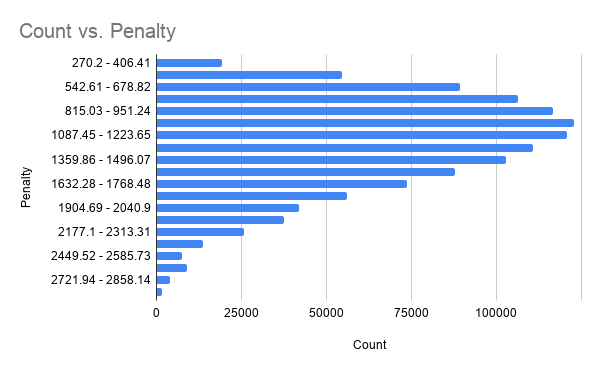
\includegraphics[width=0.65\linewidth]{figs/Count vs. Penalty.png}
    \caption{Distribution of all possible schedule scores}
    \label{fig:score_distribution}
\end{figure}

Additionally, in Table \ref{tab:brute_force_summary} brute forcing took about 3477.30ms. While this is acceptable, if the Unconference were any larger the amount of time needed to brute force would quickly become unreasonable. This is due to the search space growing at a factorial rate in relation to the number of rooms, sessions, and timeslots. However, a heuristic-based approach can be used to obtain good results without needing to search the entire space.

\section{Scheduler Results}
The scheduler was run 100 times using the same data in Table \ref{tab:session_data} to evaluate the quality and consistency of its results. In contrast to brute force search, the scheduler does not check every possible schedule. It uses local search techniques with randomness in order to find a good schedule without searching the entire search space. The results are summarized in Table \ref{tab:scheduler_results}.

  
\begin{table}[h]
\centering

\begin{tabular}{| l | r |}
\hline
\multicolumn{2}{|l|}{Scheduler Results (100 Iterations)} \\
\hline
Avg Score & 327.24 \\
\hline
Median Score & 325.00 \\
\hline
Min Score & 324.1 \\
\hline
Max Score & 340.60 \\
\hline
Avg Time (ms) & 9 \\
\hline
Min Time (ms) & 8 \\
\hline
Max Time (ms) & 12 \\
\hline

\end{tabular}
\caption{Scheduler performance over 100 iterations}
\label{tab:scheduler_results}
\end{table}

\section{Comparison}
As seen in Table \ref{tab:scheduler_results}, the scheduler produces desirable results in comparison to the distribution of all possible scores. The average, min, and max scores are all within the very top portion of the score distribution, meaning all scheduler iterations had scores that were close to optimal. Notably, even the worst schedule the scheduler produced across 100 iterations still falls within the top of the distribution of schedules. While the optimal score wasn't found, all iterations had desirable scores that did not deviate much from one another and were significantly better than the average/median score of all the schedules.

Regarding the amount of time the scheduler took to run, Table \ref{tab:scheduler_results} shows that across 100 iterations it took an average of 9ms, and with a range of 8-12ms. In comparison, it took 3,418ms for the brute force search. That means on average the scheduler had a speedup of nearly 380 times. As the problem scales, this speedup ratio also increases. To demonstrate this we can use 9 sessions from Table \ref{tab:session_data} and simulate two additional scenarios: 3 rooms with 2 timeslots and 2 rooms with 3 timeslots. 

\begin{table}[h]
\centering

\begin{tabular}{|l | l | l | l | l|}
\hline
Timeslots and Rooms & Brute Force (ms) & Scheduler (ms) & Schedules & Speedup\\
\hline
2, 3 & 4.22 & 1.55 & 1680 & 2.72\\
\hline
3, 2 & 18.22 & 1.78 & 7560 & 10.24\\
\hline
3, 3 & 3418 & 9 & 1201200 & 379.78\\
\hline

\end{tabular}
\caption{Scheduler and Brute Force Timing Scenarios}
\label{tab:scheduler_and_brute_force_timings}
\end{table}

In Table \ref{tab:scheduler_and_brute_force_timings}, there are some standouts. First, the brute force search is seeing very rapid growth in how long it takes. Similarly, the total number of schedules is seeing this same explosion of growth. Also, it shows for each scheduling scenario the multiplier for how much faster the scheduler is over brute force search. Specifically, as the scale of the schedule grows, the speedup advantage becomes significant. Something that might be surprising to see is that timeslots affect schedule time and difficulty more than rooms. This is due to the scheduler not treating the permutations of sessions within a timeslot as different schedules.

% \begin{figure}[H]
%     \centering
%     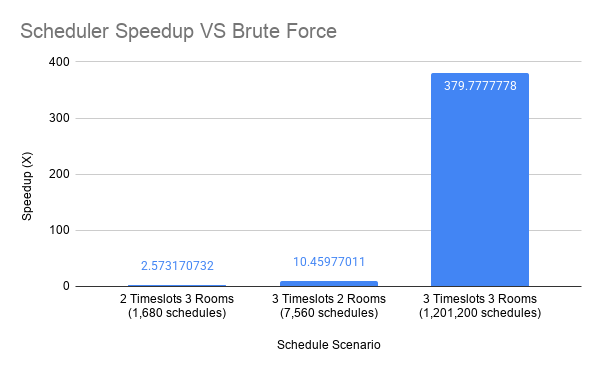
\includegraphics[width=0.75\linewidth]{figs/scheduler_speedup.png}
%     \caption{Scheduler speedup VS brute force search as the scale of the search space grows}
%     \label{fig:scheduler_speedup}
% \end{figure}

While the scheduler did not find the global optimum, it was consistently able to find schedules that were sufficiently close. For Unconference scheduling, the global optimal schedule is not required. An Unconference requires a scheduler that can provide a reasonably good schedule, while being reasonably quick to do so. The scheduler in UnconfRS has demonstrated the ability to find reasonably good schedules in a reasonable amount of time. Additionally, administrators can add schedules manually beforehand. Already determined sessions are not updated by running the scheduler.
\chapter{Conclusions and Future Work}\label{ch:conclusions}
This chapter presents the conclusions drawn from the development of UnconfRS. It revisits the two research questions regarding the use of scheduling techniques and Rust as the implementation language. This is followed by a future work section that is organized according to implementation scope and priority.

\section{Conclusions}
This thesis aimed to answer two questions: whether modern scheduling techniques can be used to create an effective Unconference management tool and whether Rust is an effective language for implementing the backend and the scheduler.

Regarding the first question, UnconfRS has demonstrated that local search with random restarts can be applied to the Unconference scheduling problem. By implementing penalty functions that account for session popularity, speaker conflicts, topic clustering, and the timing of when sessions occur, the scheduler produces reasonable schedules. However, as discussed in the future work, the penalty functions would benefit from normalization analysis. Evaluation using real Unconference data would validate that approach.

Regarding the second question, Rust proved to be well-suited for implementing the backend and the scheduler. The type system and ownership model provided compile-time guarantees that helped prevent runtime errors during development. The ecosystem was able to be leveraged with mature crates such as Axum (and various other tokio-rs crates), Askama, SQLx, Serde, and Tower to build the web application. However, Rust does come with a steeper learning curve. Some implementations become more verbose compared to conventional full-stack frameworks. With that said, the compile-time guarantees provide greater confidence in the correctness of what was implemented.

Overall, UnconfRS provides a digital Unconference management tool. It supports Unconference session proposals, session voting, and automatic schedule generation. The schedules that are generated take into account contextual information about sessions and participants to create a reasonably good result. In cases where changes need to be made, site admins have the flexibility to make manual tweaks.
%
\section{Future Work}
While UnconfRS provides a good starting point for digital Unconference management, there are areas where additional work would be beneficial. These have been organized by estimated implementation scope and priority.

\subsection{Near-Term Improvements}
These are high-priority improvements that are limited in scope and require minimal architectural changes.\\\\
%
\headerParagraph{Real-World Data}{
The current scheduler has been tested with synthetic data. Evaluating UnconfRS with data from real Unconferences would validate the effectiveness of the scheduling approach and penalty functions. This evaluation would also identify whether the heuristics align with what the organizers and participants desired. This would provide valuable data for the future work relating to the scheduling heuristics.
}\\\\
%
\headerParagraph{Scheduling Heuristics}{
Current penalty functions attempt to minimize undesirable traits in the schedule, such as having multiple popular sessions occurring at the same time, desirable sessions missing from the schedule, desirable sessions late in the day, same topics in the same time slot, and sessions that speakers want to attend happening while they are leading a session. However, these all scale differently. Some are dependent on the size of the schedule. Future work would include analysis of these heuristics to normalize their contributions to the overall score.
}\\\\
%
\headerParagraph{Multi-Threaded Scheduling}{
Currently the scheduler runs its random restarts sequentially, with each restart running an iteration of scheduling before the next begins. The runs are independent of one another and is parallelizable. Future work could add optional multi-threading to run these in parallel if the user desired.
}\\\\
%
\headerParagraph{Frontend Enhancements}{
The current frontend, based on Askama templates, Bootstrap, and the HTML 5 drag and drop API, provides the main functionality but leaves room for improvement. Accessibility enhancements are an area that would benefit UnconfRS. The ability for session creators to record attendance and notes within this platform is a logical inclusion. Additionally, the application currently makes use of browser alert popups. These should be replaced with Bootstrap alternatives.
}
%
\subsection{Longer-Term Improvements}
These are either lower priority improvements or require a larger effort.\\\\
%
\headerParagraph{Alternative Scheduling Methods}{
In its current implementation, UnconfRS utilizes local search. Analysis of a variety of alternative scheduling methods would provide a clearer idea of what the best approach is. The best approach might vary from Unconference to Unconference as well. For new methods implemented, they should be able to be conditionally enabled through an environment variable. 
}\\\\
\headerParagraph{Registration}{
Improve the UnconfRS registration workflow.
}\\\\
%
\headerParagraph{Frontend Rewrite}{
Since the backend of UnconfRS is written in Rust, rewriting the frontend using a Rust-based framework would unify both to be written in the same language. This would allow data structures to be shared between the frontend and backend, removing potential inconsistencies. Additionally, a Rust-based frontend would benefit from compile-time guarantees and the type system.
}
\chapter{Availability}\label{ch:availability}
The source code uses the MIT license and is available at \hyperlink{UnconfRS}{https://github.com/relia1/UnconfRS}
% \chapter*{Bibliography}

\bibliography{thesis}
\bibliographystyle{ACM-Reference-Format}
\end{document}